
%%%%%%%%%%%%%%%%%%%%%%%%%%%%%%%%%%%%%%%%%%%%%%%%%%%%%%%%%%%%%%%%%%% 
%                                                                 %
%                           INTRODUCTION                          %
%                                                                 %
%%%%%%%%%%%%%%%%%%%%%%%%%%%%%%%%%%%%%%%%%%%%%%%%%%%%%%%%%%%%%%%%%%% 
 
\chapter{INTRODUCTION}
\label{chapter:intro}

% magical first sentence
% explain like you would to your parents/non-technological people
% - explain how keyframe animation currently works
% explain in more technical terms what this means
% - problems with current techniques
% - what can be done (auto animation)
% - overview of controllers
% - overview of the technique
Animations of human characters are used heavily in video games, movies, and other fields.  Especially with the increasing usage of complex environment traversal in both film and video games, many similar animations of athletic motions must be created with small changes to tune the motion to the particular situation, environment, and character.  Creation of such animations is largely done by hand by artists using keyframing.  In a keyframe animation, certain ``key'' parts of the animated sequence are specified, with the remaining frames filled in, or ``tweened'' using an automated interpolation method or manual frame addition.  For 2D animation, this occurs as a series of images which are played back in order to produce the animation.  In 3D, keyframe animations are performed on a 3D model.

% figure of sprite animation frames
\begin{figure}[htp]
    \centering
    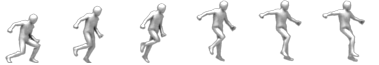
\includegraphics[width=\textwidth]{images/sprite_example/platformer_sprites_jump.png}
    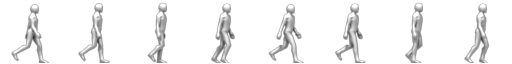
\includegraphics[width=\textwidth]{images/sprite_example/platformer_sprites_walk.png}
    \caption[Example of a 2D Sprite Animation]{This example shows a 2D sprite sheet used to produce a jumping animation for a stick figure character.  The frames in this case are laid out in a single image for demonstration purposes, progressing in order starting with frame 0, the frame farthest left in this sprite sheet.}
    \label{fig:sprite_sheet}
\end{figure}

3D models are described as a mesh, a collection of primitive polygons (i.e. quadrilaterals or triangles) which are stored as vertices.  This mesh describes what is drawn, including any texture, color, and other material information.  Along with the mesh, a skeleton, or rig, is stored.  The rig describes a heirarchical structure of bones and accompanying joints.  Each vertex is given a series of weights describing the impact each joint has on its transformation.  This allows many vertices, and therefore many polygons, to be transformed at once in organized groups, simplifying the problem of animating the model to a matter of transforming the skeleton in the desired manner.  To animate this 3D model, an artist specifies keyframes of the animation by positioning the skeleton at different time steps.  The stored keyframes, instead of an image, are the transformations of each joint at this frame or step of the animation, which a rendering or game engine can interpolate between to produce the final result.

%TODO make the images the same level of zoom
\begin{figure}[htp]
	\centering
	\begin{subfigure}[b]{0.41\textwidth}
		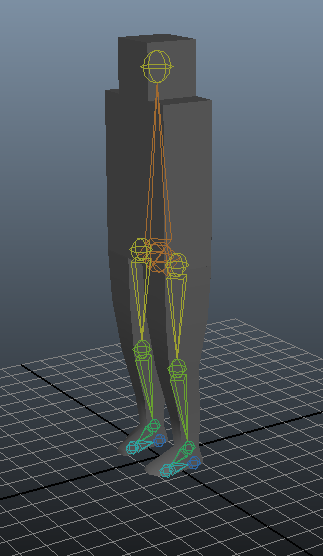
\includegraphics[width=\textwidth]{images/simpleSkeleton2Screen1Cropped.png}
	\end{subfigure}
	\begin{subfigure}[b]{0.3\textwidth}
		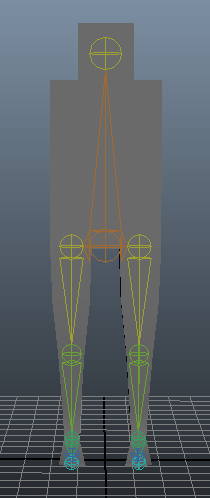
\includegraphics[width=\textwidth]{images/simpleSkeleton2Screen2Cropped.png}
	\end{subfigure}
	\caption[Example of Rigged 3D Character Model]{Above is an example of a character model in \maya.  The character skin or mesh is shown in gray, with a rig shown in multicolor.  While it is visualized as a series of spherical joints with connecting solids, the rig itself does not have a visual component in practice.  The rig acts as a skeleton, deforming the mesh of the character model to make animation easier.  Additional tools such as deformer groups and inverse kinematics handles can be used to further simplify the creation of animations for artists.  While these tools simplify movement of the model, the artist still must position each joint for each frame of the animation, which is then stored for later playback.}
	\label{fig:rig_character}
\end{figure}

Specifying these animation frames is work intensive, taking up significant time and resources to produce for a single character.  Additionally, similar animations may need to be produced for slightly different scenarios, with only minor modifications required.  These minor modifications can be to fit a different setting, such as a character jumping on Earth or on the moon, or can be for different characters, such as a large person moving in contrast with a small child.  Though the movement itself may be similar, manual changes must be made, requiring artist time which could be spent generating new assets.  

Recent work in animation generation seeks to automate this process, replacing the manual process with a procedural one.  Physics based simulations can be used to produce controllers for the skeleton, determining joint positions and rotations for keyframes automatically.  Not only does this reduce the effort involved in the creation process, but this also provides a basis for dynamic interaction between a character's animation and the environment, which is not possible with manual keyframe animations.

We present a controller that takes a skeleton as input, with additional parameters describing the character, which produces a sequence of poses for a keyframe animation.  The additional character parameters describe the character's mass as well as the constraints placed on each joint to prevent unnatural rotations.  Weight is specified per-joint to allow for calculation of the character's center of mass.  Our controller works with the initial flex and takeoff stage of the jumping motion.  The motion is calculated by modeling muscles as simple springs attached to the skeleton at 2 points.  Spring constants for the muscles are determined by the user, which are applied in a linear spring calculation to determine the approximate change from rest length required to achieve a particular force.  This change from rest length approximates the flexion required, which can be used to calculate a plausible amount of bend for the wind-up motion of a jump.

To control the motion and maintain plausibility, calculations are performed to determine the character's center of mass and supporting polygon.  As the character should maintain balance while flexing its joints, the position of the character's joints are adjusted to keep the center of mass positioned over the supporting polygon.  Flexion proceeds with the character bending progressively, maintaining balance while moving to achieve the desired spring force in its leg muscles.

The next stage of the motion, the take-off where the character releases from the ground, uses the potential energy of the spring-muscles and accelerates the character's center of mass upward.  Application of force works from the joints and muscles closest to the center of mass outwards through the skeleton.  While not handled by our controller, the character would then proceed through the in-air portion of the jump, where the acceleration changes due to gravity as well as other forces before they finally land.  We assume a simple trajectory for the in-air phase, though more complex motions with turns, flips, or interaction with the environment could be created.  Other work has handled landing with a similar approach. \cite{falling_landing}

Our controller is made to be a module, able to be used with other controllers as part of a larger system.  This allows each controller to do a smaller job well. Several such controllers can be connected to produce more complex animations or animation sequences, utilizing bounded starting and finishing conditions for the character. Additionally, certain cases during the duration cause the controller to stop early, for example a mid-air collision mid jump which would require a separate controller to handle this case. \cite{composable_controllers}

% figure of current keyframe animation process in maya
% accompanying video for presentation
% accompanying figure/video of the resulting animation in 3d

\section{Setup and Inputs}
The character in our system consists of a mesh, a skeleton, and a controller which has itself several sub-components.  First we constructed a mesh, a 3D visual representation of our character.  Our mesh is a simple, blocky humanoid, lacking arms in order to focus more heavily on the lower body motion of the figure.  A more complex human character, or even a humanoid non-human character could be substituted.  This mesh consists of vertices, which each have a position as well as other information not relevant to our simulation such as normal and texture coordinate, which are used by \unity for displaying the mesh.  This mesh can also be referred to as a character model, but in the context of this simulation we will refer to it as the mesh.  Three vertices form a triangular face, though these are often created as quadrilaterals by the artist as the topology of the model can be simpler to work with due to the grid patterns formed as compared to triangular meshes.  In the case of quad meshes, the mesh is often treated as a triangle mesh by the game engine or renderer, with each quad producing two triangles.

Our mesh was created using \maya, positioning the vertices in groups or individually, using several rectangular prisms as a base.  Using the edge loop tool, more vertices were inserted, with loops of edges circling the torso and legs to produce the final shape.  This mesh was then rigged, meaning a skeleton was added.  As described in further detail in \ref{subsection:skel_joints}, joints were positioned individually relative to the mesh, attempting to mimic the positioning of joints in the human skeleton.  The connections were made simply, with each joint acting as a ball and socket joint, meaning that constraints needed to be specified at a later stage to facilitate hinge joints such as the knee and ankle and that complex, multi-boned structures as found in the foot and shin were simplified to a single bone connecting two joints.  The hierarchy of joints for the skeleton was rooted at the pelvis with three children: one leading to the upper body and one to each hip.  From there a single joint was used for the manipulation of the upper body, with separate joints for each hip, knee, ankle, toe, and heel.  Though there is no movement in the toe, placing a bone for the foot requires an end joint for the bone to connect to.

%TODO how do i talk about this with authority, there isn't really anything to cite there's just youtube videos and it's generally taught as such/discovered via industry
Joints are then associated with the mesh through weight painting, in which each vertex of the mesh is assigned a weight for each joint.  This weight designates if and how much a vertex transforms when a joint is moved.  Each vertex must be assigned a weight for each joint of the model.  Careful weight assignment is highly important as this determines the behavior of the character's ``skin'' when they move, affecting how the mesh twists or bends as well as which parts move with which bones.  The joints may then be used to manipulate the mesh to produce animations, with each keyframe in an animation storing information about each joint instead of each vertex.

\subsection{User Specified Constants}
\label{subsection:user_constants}
% specified constants
% gravity
% air time
% windup time
% error allowance (between calculated skeleton values and desired)
% drag
% jumping policy (not implemented)
% Windup PD k values
% Balance PD k values
% muscle values foreach muscle:
%	k (linear spring constant)
%	anchor joints (for our simulation, 2)
% 	center joint
%   [0,1] scale to indicate muscle anchor position (0 is closer to center joint, 1 is closer to end joint)
%   bone width
% calculated values
Within the controller there are a number of constants the user can specify, outside of the character itself.  These specify constants for the simulation environment as well as some constants describing the animation to be produced.  Our only environmental constant is gravity, which we specify as -10 $\frac{m}{s^2}$, where the negative indicates the downward direction.

\subsection{Skeleton, Joints, and Muscles}
\label{subsection:skel_joints}
For the purposes of animation, a joint is an object with an associated position, associated transformation, a parent joint, and some number of child joints.  In the case of the root, the parent joint is absent and in the case of the end joints such as tips of the fingers there are no child joints.  Each child joint is connected to the parent by a rigid bone, which protrudes from the parent at a given resting angle.  These joints are structured in a tree, as the parent and child joints imply, with the root of the tree at the pelvis.  This tree serves as a hierarchy for transformations.

Joints are associated with a set of vertices from the mesh to be animated.  Each of these may be associated with multiple joints, and are assigned a weight for each joint which acts as a scale factor for the transformations performed on the vertex.  When a joint is transformed, the transformation is propagated to the children, with the parent as the origin of the child node's coordinate system.

\section{An Example of Animation Creation}
To motivate the necessity for an automated animation method, we present an example of the method for producing an animation by hand.  

% explain contributions
% - what is the contribution of this technique
% - Unity3D -> what am I getting from outside sources
% - what am I making myself
\section{Contributions}
	This thesis describes a controller which simulates a jumping motion on a character.  The generated animation is created to be plausible in appearance, though it may not be a physically accurate representation.  Specifically, we contribute a model for the windup and take-off phases of a jump and created a controller using this model in \unity.

	\unity is a game engine which we used to develop this system.  It provides infrastructure for rendering, scene management, skeletal animation, asset import and management, lighting, and scripting.  The system developed leverages the provided features through the \unity scripting interface.  We developed scripts for calculation of muscle forces, as well as for applying the force to an imported model.  Models were created in \maya and imported using \unity's asset import as \unity game objects with attached Transform components which allow arbitrary transformations.
